\subsection{The Capacitive Memory Window and Its Frequency Collapse}
GIXRD [Fig.~\ref{fig:stacks}(b)] shows the dominant polar orthorhombic
reflection near $2\theta \approx 30.4^\circ$ with a residual monoclinic
contribution near $28.5^\circ$, confirming both films as ferroelectric
\hzo{}~\cite{boscke2011,muller2012,iung2025}. Fig.~\ref{fig:stacks}(c)
summarizes the wake-up transformation for
reference~\cite{pesic2016,schenk2014,grimley2016,cho2024wakeup}.

Fig. 2(a) shows the effective permittivity of Stack~A at
1~kHz for both sweep directions. The butterfly peaks reach
$\xir \approx 62$ near $\mp0.55$\MVcm{}, and the two branches do not coincide
at zero field: $\xi_\downarrow(0) = 55.0$ and $\xi_\uparrow(0) = 49.8$,
giving $\CMW_\xi \approx 5.2$. This splitting---read at zero bias without
disturbing the stored state---is the capacitive memory window. Stack~B
[Fig. 2(b)] reaches the same peak permittivity,
$\xir \approx 62$, but gives $\CMW_\xi \approx 2.3$ at the same 1~kHz probe
frequency.

Fig. 2(c) and (d) follow the frequency dependence for Stack~A
and Stack~B respectively. For Stack~A (c), from 1~kHz to 400~kHz two things
occur together: the peaks fall from 62 to 30, and the branch separation
shrinks until, by 400~kHz, the window has essentially closed. Critically, the
dielectric response itself does not vanish---a permittivity of $\approx$30
persists at 400~kHz and $\approx$27 at 500~kHz. What disappears is the
\emph{difference} between the states. Stack~B (d) shows the same behaviour but
at a far lower corner: because its window closes near 1.4~kHz, the branches
have already merged across the entire 50--400~kHz range shown, and the two
sweep directions are nearly coincident at every frequency. In both stacks the
window is therefore carried by a dispersive contribution superposed on a
largely non-dispersive background---the same process at two very different
corner frequencies, previewing the two-clock comparison of
Fig. 4---motivating the two-component treatment below.
\begin{figure}[H]
     \centering
     \begin{subfigure}[b]{0.49\columnwidth}
          \centering
          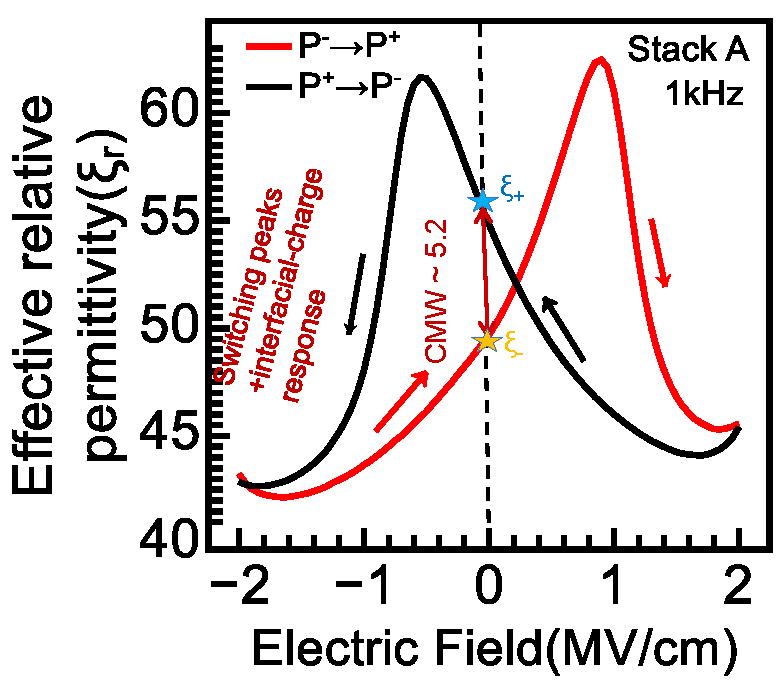
\includegraphics[width=\textwidth]{figures/fig 2a.pdf}
          \caption{}
          \label{fig:fig1a}
     \end{subfigure}
     \hfill
     \begin{subfigure}[b]{0.49\columnwidth}
          \centering
          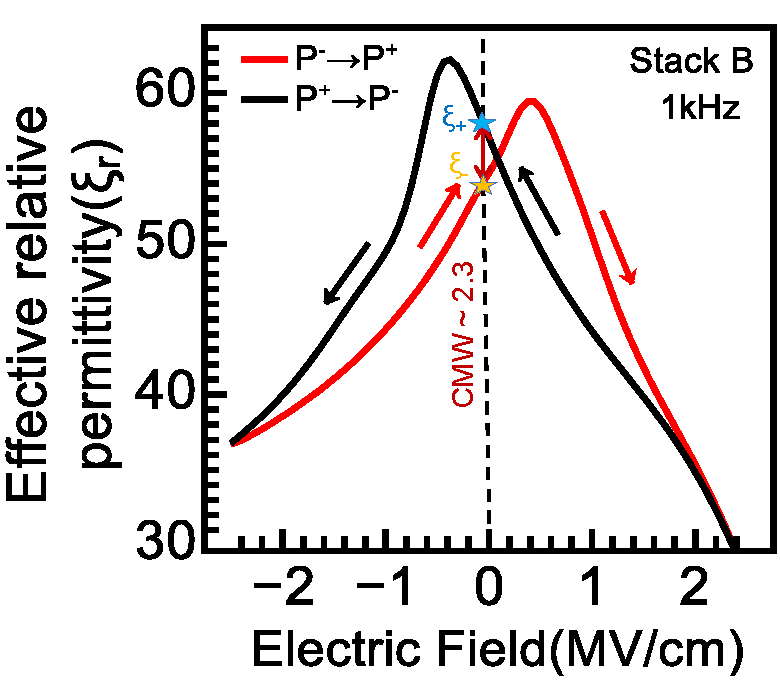
\includegraphics[width=\textwidth]{figures/fig 2b.pdf}
          \caption{}
          \label{fig:fig1b}
     \end{subfigure}
      \hfill
     \begin{subfigure}[b]{0.49\columnwidth}
          \centering
          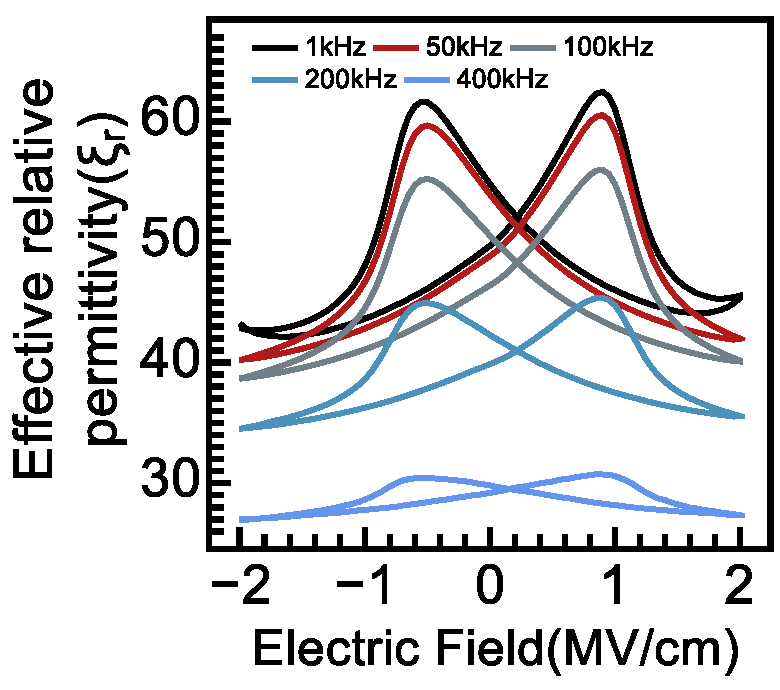
\includegraphics[width=\textwidth]{figures/fig 2c.pdf}
          \caption{}
          \label{fig:fig1c}
     \end{subfigure}
           \hfill
            \begin{subfigure}[b]{0.49\columnwidth}
          \centering
          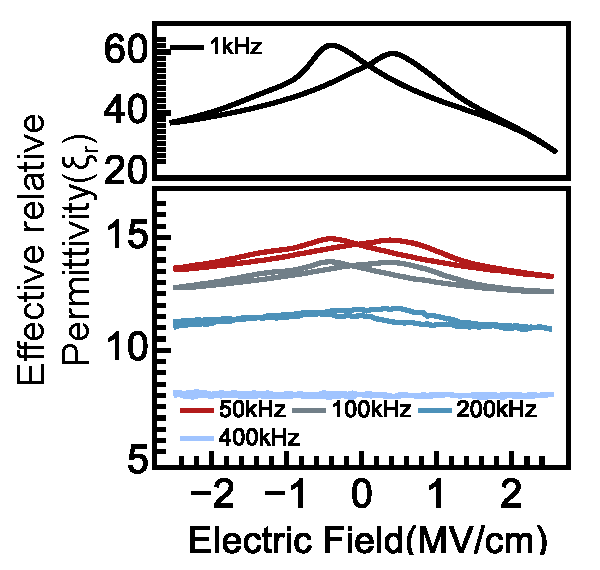
\includegraphics[width=\textwidth]{figures/fig 2d.pdf}
          \caption{}
          \label{fig:fig1c}
     \end{subfigure}
           \hfill
     
     
     \caption{Definition and frequency collapse of the CMW at 300~K.
(a) Effective relative permittivity of Stack~A at 1~kHz for both sweep
directions; the branches are displaced at zero field,
$\xi_\downarrow(0) = 55.0$ and $\xi_\uparrow(0) = 49.8$, defining
$CMW_\xi \approx 5.2$. (b) The same measurement on Stack~B, giving
$CMW_\xi \approx 2.3$ at the same peak permittivity. (c) Stack~A from 1~kHz
to 400~kHz; the branch separation collapses while a permittivity of
$\approx$30 remains at 400~kHz, indicating that the window is carried by a
dispersive contribution superposed on a largely non-dispersive background.(d)The same frequency series for Stack B; the window closes at far lower frequency, consistent with its lower corner.}
     \label{fig:figure1}
\end{figure}



\subsection{The Interface Sets the Clock}
If the window is interface-limited, changing the interface should change its
dynamics; if ferroelectric-limited, it should not.

\textit{Identical ferroelectric ceilings.} Fig. 3(c) shows
the peak permittivity of both stacks. Extrapolating the roll-off to zero
frequency using the same Debye form gives $\xir(f\!\rightarrow\!0) =
62.4 \pm 1.2$ for Stack~A and $62.7 \pm 0.9$ for Stack~B---statistically
identical, and consistent with the measured 1~kHz values of 62.5 and 62.2.
Both stacks therefore present the same intrinsic dielectric amplitude from
the \hzo{} layer. Their high-frequency limits differ,
$\xi_\infty = 21.7 \pm 0.9$ and $15.8 \pm 0.5$, as expected if the series
interfacial layers differ. (Stack~B's apparent decline to $\xir \approx 6$
above 200~kHz falls below its own fitted $\xi_\infty$ and is circuit-limited,
its larger capacitance placing its RC corner lower.)

\textit{Two-decade difference in clock.} Against those identical ceilings,
the two windows relax $126\times$ apart in relaxation time,
$\tau = 0.90\,\mu$s versus 114~$\mu$s, from the single-Debye fits detailed in
Section~III-D. Fig. 3(d) shows that scaling each dataset by
its own corner frequency and plateau collapses both onto the universal Debye
form $1/(1+x^2)$---the same functional response, two different clocks.
Fig. 5(e) summarizes: identical dielectric response (62
versus 62), windows of 5.2 versus 2.4 at 1~kHz, and built-in fields of 0.22
versus 0.08\MVcm{}. The stack with the larger built-in field also shows the
larger window, consistent with the asymmetry setting the window amplitude,
although two devices cannot establish a scaling relation between them.

\textit{Controls.} First, Stack~B's low corner is not an RC artifact: with
the fitted $R_s$ and Stack~B's capacitance the circuit-limited corner lies
near 220~kHz, more than two decades above the observed 1.4~kHz. Second, the
difference cannot originate in the ferroelectric, whose low-frequency
dielectric ceiling is identical in both to within 1.5\%.

We attribute the difference to the interface, noting the structural
correlation that Stack~B, which contains a deliberate WO$_x$ interfacial
layer~\cite{paul2026wox}, is the slower of the two---as expected for
relaxation across a more resistive interfacial layer. We state the limitation
explicitly: the two stacks differ in electrode materials and ferroelectric
thickness as well as in the WO$_x$ layer, so a single causal variable cannot
be isolated from two devices. The claim the data support unambiguously is
that two stacks sharing the same ferroelectric dielectric ceiling exhibit
windows differing by two orders of magnitude in relaxation time---the clock
is not set by the ferroelectric.

\subsection{Mechanism: Maxwell--Wagner Relaxation}
A ferroelectric layer in series with a thinner, more resistive interfacial
layer exhibits Maxwell--Wagner interfacial relaxation with a single time
constant~\cite{jonscher1983,kremer2003}
\begin{equation}
\tau = \frac{\varepsilon_i d_f + \varepsilon_f d_i}
            {\sigma_i d_f + \sigma_f d_i}
     \;\approx\; \frac{\varepsilon_i}{\sigma_i}
     \qquad (d_i \ll d_f)
\label{eq:mw}
\end{equation}
set by the interfacial layer alone [Fig. 3(a)]. This
accounts for every observation without additional assumptions.

A two-layer series network produces exactly one relaxation, matching the
single-Debye character established in Section~III-D (the undepressed
Cole--Cole arc of Fig. 4(c) and the 2\% agreement among
three independent corner determinations). The interfacial layer supports a
static built-in potential set by the electrode/oxide chemistry, giving the
frequency-independent $\Ecross$ above while the charge redistribution across
it relaxes. Because $\tau$ depends only on the interfacial layer, it changes
with the stack: taking $\varepsilon_i$ from the measured $\xi_\infty$ values,
\eqref{eq:mw} implies $\sigma_i = 2.2\times10^{-4}$~S/m for Stack~A and
$1.2\times10^{-6}$~S/m for Stack~B. These are order-of-magnitude estimates,
but they lie in the range expected for a defective, vacancy-rich interfacial
oxide~\cite{kim2023vacancy,segantini2023strain,koroleva2022,iung2025}, and
their ratio reproduces the observed spread in $\tau$. The picture is
independently supported by impedance spectroscopy of 10~nm \hzo{} capacitors,
which resolves distinct interface and bulk RC elements with pristine
resistances of $\approx$1~k$\Omega$ and $\approx$500~M$\Omega$
respectively~\cite{alcala2023}. Since $\sigma_i$ is thermally activated,
$\tau$ grows rapidly on cooling and the corner falls out of the measurement
band, as shown in Section~III-E [Fig.~\ref{fig:temperature}(e)], while the
ferroelectric---whose switching does not depend on interfacial
conduction---continues to operate.


\textit{Separating the interfacial capacitance from the interfacial
resistance.} Because the interfacial region enters as a series element, its
areal capacitance can be extracted directly from the two permittivity limits
without any assumption about its thickness or permittivity. Writing the
low-frequency limit $\xi_{FE}$ (interfacial layer conducting) and the
high-frequency limit $\xi_\infty$ (interfacial layer blocking) as series
capacitances gives
\begin{equation}
c_{IL} = \frac{\varepsilon_0}{d\left(\xi_\infty^{-1}-\xi_{FE}^{-1}\right)},
\qquad
R_{IL} = \frac{\tau}{c_{IL}}
\label{eq:cil}
\end{equation}
the second relation following from $\tau = R_{IL}c_{IL}$ for the series
element. Applying \eqref{eq:cil} to the fitted limits gives
$c_{IL} = 2.95$ and 2.34~$\mu$F/cm$^2$ for Stacks~A and~B [Fig. 3(b)], while the
corresponding areal resistances are 0.30 and 48.6~$\Omega\cdot$cm$^2$, a
factor of $\sim$160. The product reproduces the measured relaxation times
exactly ($R_{IL}c_{IL}$ ratio $= 128$ versus the observed $\tau$ ratio of
128), confirming internal consistency. The interfacial capacitances are
comparable---their ratio is 1.3 as measured, or 1.6 when both are referred to
a common thickness, since $c_{IL}$ scales as $1/d$ and the two films differ in
thickness---whereas the interfacial resistances differ by more than two orders
of magnitude. The WO$_x$-bearing stack is therefore slower by virtue of
interfacial \emph{resistance}, not interfacial capacitance or thickness
[Fig. 3(b)]. This is a design statement---to move the read
corner, engineer interfacial conductivity---and it is obtained without imaging
the interface. This is a design statement---to move the read corner, engineer
interfacial conductivity rather than interfacial thickness---and it is
obtained without imaging the interface. We note that $c_{IL}$ and $R_{IL}$
are sums over both interfaces of each stack and cannot be apportioned between
them electrically; converting them to a physical thickness additionally
requires $\xi_{IL}$, for which $\sigma_i \approx 10^{-6}$--$10^{-4}$~S/m
follows if $\xi_{IL} \approx 6$--30 is assumed.

This does not imply the ferroelectric is absent from the window: below $\fc$
the measured capacitance is that of the ferroelectric layer, and the
polarization defines the two states being compared. It implies that the
window's \emph{existence} requires the interfacial asymmetry, and that its
magnitude, clock and temperature range are interfacial properties.
\begin{figure}[H]
     \centering
     \begin{subfigure}[b]{1\columnwidth}
          \centering
          
\includegraphics[width=\textwidth]{figures/figure3/fig 3a.pdf}
          \caption{}
          \label{fig:fig1a}
     \end{subfigure}
     \hfill
     \begin{subfigure}[b]{0.49\columnwidth}
          \centering
          
\includegraphics[width=\textwidth]{figures/figure3/fig 3b.pdf}
          \caption{}
          \label{fig:fig1b}
     \end{subfigure}
      \hfill
     \begin{subfigure}[b]{0.48\columnwidth}
          \centering
          
\includegraphics[width=\textwidth]{figures/figure3/fig 3c.pdf}
          \caption{}
          \label{fig:fig1c}
     \end{subfigure}
           \hfill
           \begin{subfigure}[b]{0.49\columnwidth}
          \centering
          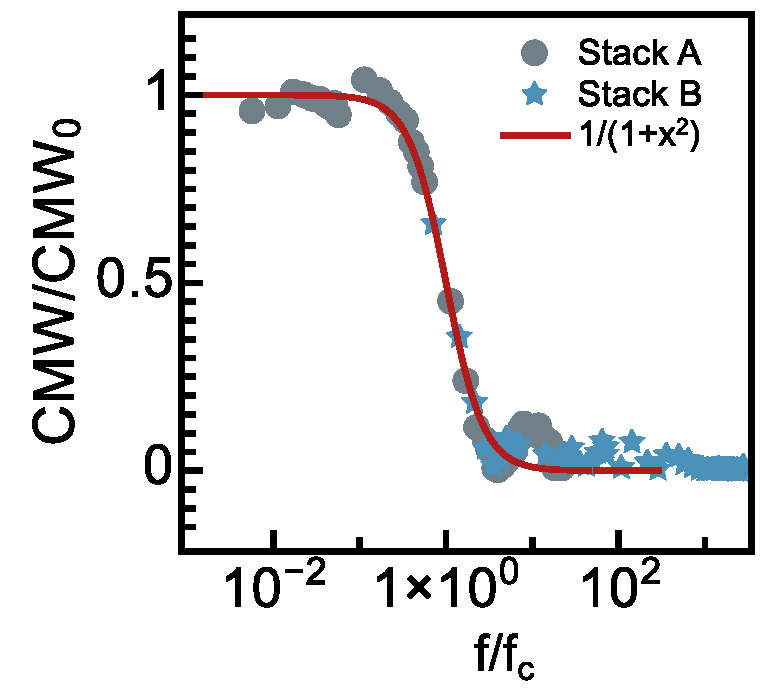
\includegraphics[width=\textwidth]{figures/figure3/fig 3d.pdf}
          \caption{}
          \label{fig:fig1c}
     \end{subfigure}
           \hfill
             \begin{subfigure}[b]{0.49\columnwidth}
          \centering
          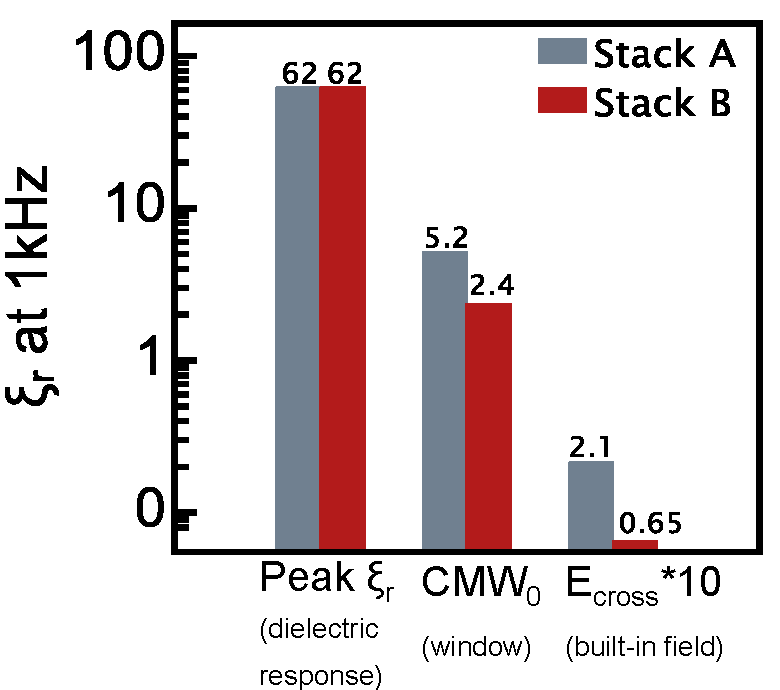
\includegraphics[width=\textwidth]{figures/figure3/fig 3e.pdf}
          \caption{}
          \label{fig:fig1c}
     \end{subfigure}
           \hfill
     
     
     \caption{Interfacial origin of the capacitive memory window.
(a) Cross-sections of both stacks including the reacted interfacial regions:
TaO$_x$N$_y$ and TiO$_x$N$_y$ form at the nitride contacts of Stack~A and at
the PE-TiN contact of Stack~B by oxygen scavenging during deposition and
crystallization.(b) Interfacial areal capacitance $c_{IL}$ and resistance $R_{IL}$
extracted from the dispersion limits via \eqref{eq:cil}: the two stacks have
comparable $c_{IL}$ but differ by $\sim$160$\times$ in $R_{IL}$, so the
WO$_x$-bearing stack is slower by virtue of interfacial resistance, not
capacitance or thickness. (c) Peak permittivity versus frequency; both stacks
extrapolate to the same low-frequency dielectric ceiling, $\xir(f\!\to\!0)
\approx 63$, while their high-frequency limits differ ($\xi_\infty = 21.7$ and
15.8). (d) Master-curve collapse: scaling each dataset by its own corner
frequency and plateau collapses both stacks onto the parameter-free Debye form
$1/(1+x^2)$---the same functional response, two different clocks. (e) Summary
comparison of dielectric response, window magnitude and built-in field for the
two stacks.}
     \label{fig:figure1}
\end{figure}

We present
this as the interpretation consistent with all measurements; the oxygen-vacancy population underlying the interfacial charge is
confirmed directly by O~1s XPS [Fig.~\ref{fig:stacks}(d)], while the spatial
location and thickness of the reacted interfacial layer remain to be resolved;
direct structural confirmation by TEM/EELS of the two
interfaces~\cite{iung2025,kumar2025review,das2026paradox} is the natural next
step.

\subsection{The Window Relaxes as a Single Debye Species}
\label{sec:debye}
We model the poled stack as a two-component dielectric,
\begin{equation}
\xi^{*}_{\pm}(\omega) \;=\; \xi_\infty + \frac{\Delta\xi_\pm}{1+j\omega\tau}
\label{eq:twocomp}
\end{equation}
where $\xi_\infty$ is the polarization-independent high-frequency
permittivity and $\Delta\xi_\pm$ the state-dependent relaxing term. Because
$\xi_\infty$ cancels analytically in the difference between states, the
measured window isolates the relaxing component and is insensitive to the
large non-relaxing background:
\begin{align}
\CMW(f) &= \frac{\CMW_0}{1+(f/\fc)^2} \label{eq:debyereal}\\
\Delta\xi''(f) &= \frac{A_{\mathrm{DC}}}{f}
   + \CMW_0\,\frac{f/\fc}{1+(f/\fc)^2} \label{eq:debyeimag}
\end{align}
with $\fc = 1/2\pi\tau$. The first loss term accounts for a state-dependent
DC leakage contribution~\cite{nicollian1982,schroder2006}.

\textit{Real part.} Fig. 4(a) shows the measured CMW for
both stacks across 61 frequencies. Stack~A is described by
\eqref{eq:debyereal} with $\CMW_0 = 5.38$ and $\fc = 179$~kHz, corresponding
to $\tau = 0.90\,\mu$s. Stack~B gives $\CMW_0 = 3.6$ and $\fc = 1.4$~kHz,
i.e.\ $\tau = 114\,\mu$s; because Stack~B's roll-off begins below 10~kHz its
plateau is an extrapolation, and its measured 1~kHz value (2.36) already lies
at $f/\fc = 0.71$ on the roll-off.

\textit{Imaginary part.} Fig. 4(b) fits
\eqref{eq:debyeimag} to the differential loss of Stack~A, obtained
independently from the conductance channel. The decomposition returns a
leakage coefficient $A_{\mathrm{DC}} = 551$~Hz and a Debye peak at
$\fc = 182$~kHz with amplitude 5.94---within 2\% of the real-part corner. The
residual is 0.13 against a peak loss of 2.9.

\textit{Cole--Cole locus.} Fig. 4(c) presents the
differential Cole--Cole plot over 30--300~kHz after removal of the leakage
term. Below 30~kHz the subtraction dominates the signal and above 300~kHz
series-resistance loss lifts the locus; those points are shown as open
symbols and excluded from the fit. The circular-arc fit constrained to pass
through the origin returns a depression angle $\alpha = -2.7^\circ$, zero
within uncertainty and of unphysical sign, so $\beta = 1$ within resolution.
Forcing an ideal Debye arc with its centre on the real axis increases the rms
radial residual only from 3.1\% to 3.5\% of the radius, so a distribution of
relaxation times is not required by the data. The arc amplitude, 5.50, agrees
to 2.1\% with $\CMW_0 = 5.38$ from the real-part fit---Kramers--Kronig
closure between two independent measurement channels~\cite{colecole1941}.

Three determinations of the corner---179~kHz (real part), 182~kHz (loss peak)
and the arc geometry---agree within 2\%. The window relaxes as one
well-defined species, which a distributed domain-wall or defect-continuum
response would not produce~\cite{jonscher1977,jonscher1983}.

\textit{Completeness of the relaxation.} Admitting a non-relaxing offset,
$\CMW(f) = \CMW_\infty + \CMW_0/[1+(f/\fc)^2]$, returns
$\CMW_\infty = -0.36 \pm 0.11$, negative and therefore unphysical as a
residual; any non-relaxing component is below 7\% of $\CMW_0$. This is
significant because a window limited by the ferroelectric's own response,
which persists into the GHz range~\cite{kim2023impedance}, would leave such a
residual. Instead, at 500~kHz the window has fallen to 0.45 while the
permittivity is still 27: what survives the relaxation is state-independent.

\textit{Intrinsic origin of the corner.} With $R_s = 267\,\Omega$, the
circuit-limited corner lies at 1.81~MHz and the correction factor
$(\omega R_s C)^2 = 0.010$ at $\fc$. The 179~kHz corner is therefore a
property of the device, not the measurement circuit.

\begin{figure}[H]
     \centering
     \begin{subfigure}[b]{0.49\columnwidth}
          \centering
          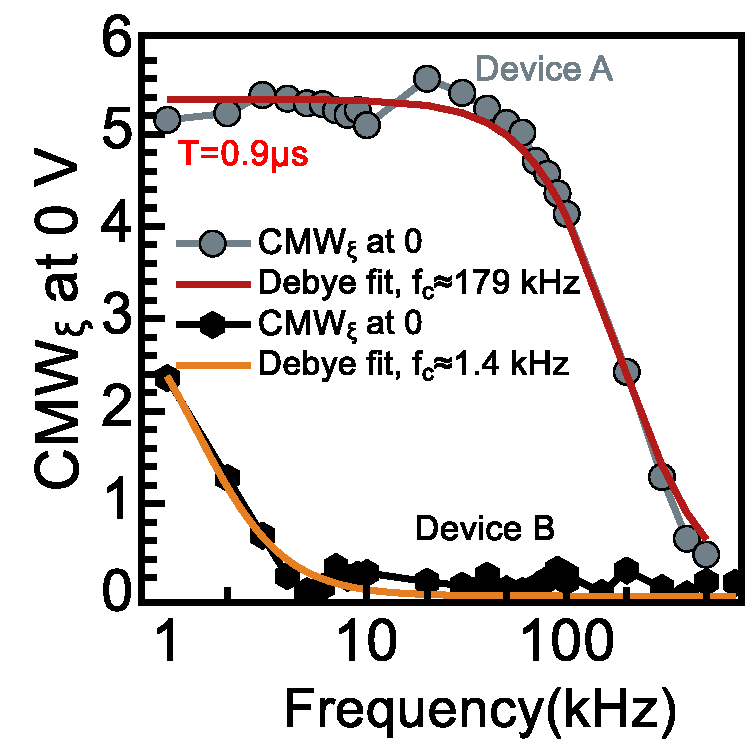
\includegraphics[width=\textwidth]{figures/fig 3a.pdf}
          \caption{}
          \label{fig:fig1a}
     \end{subfigure}
     \hfill
     \begin{subfigure}[b]{0.49\columnwidth}
          \centering
          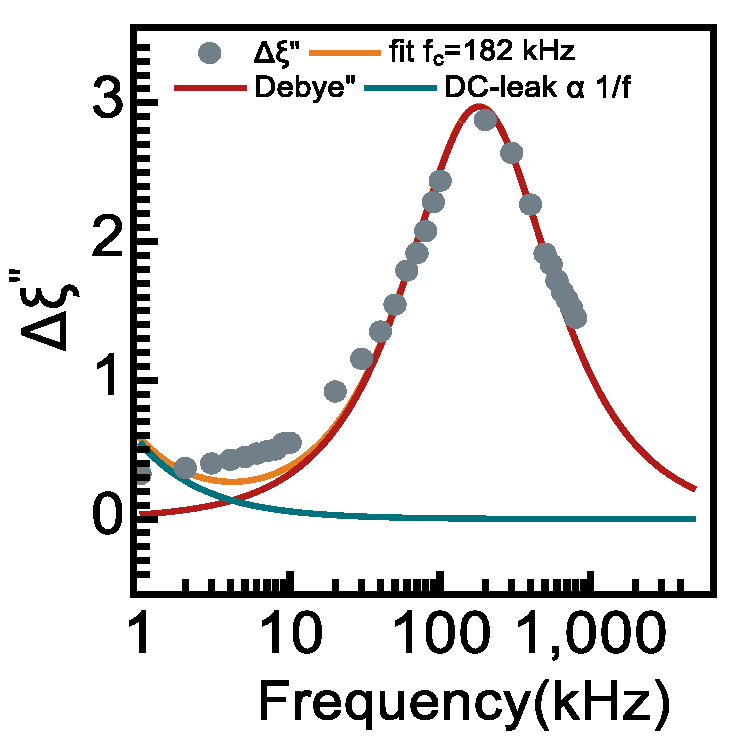
\includegraphics[width=\textwidth]{figures/fig 3b.pdf}
          \caption{}
          \label{fig:fig1b}
     \end{subfigure}
      \hfill
     \begin{subfigure}[b]{0.63\columnwidth}
          \centering
          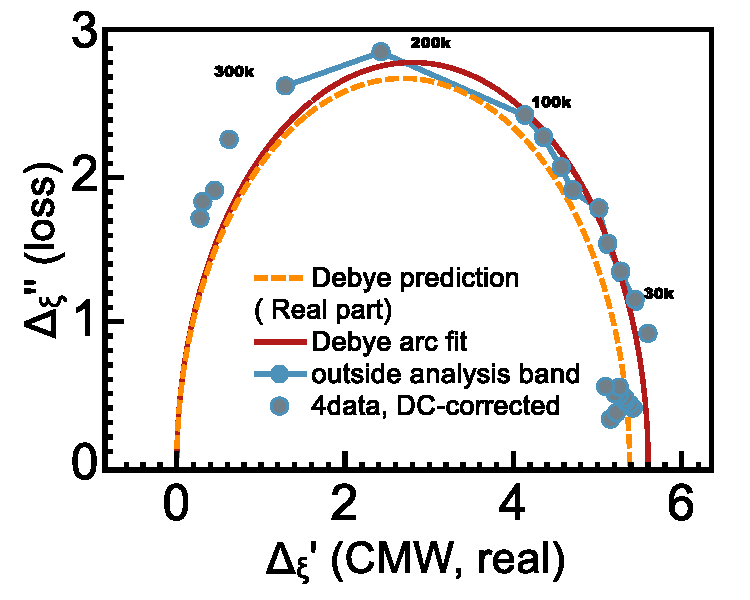
\includegraphics[width=\textwidth]{figures/fig 3c.pdf}
          \caption{}
          \label{fig:fig1c}
     \end{subfigure}
           \hfill
     
     \caption{The window relaxes as a single Debye species. (a) CMW at zero bias
versus frequency for both stacks with single-Debye fits: $f_c = 179$~kHz
($\tau = 0.90\,\mu$s) for Stack~A and $f_c = 1.4$~kHz ($\tau = 114\,\mu$s)
for Stack~B. (b) Differential loss $\Delta\xi''$ for Stack~A, decomposed into
a DC-leakage contribution $\propto 1/f$ and a Debye loss peak at 182~kHz,
obtained from the conductance channel and therefore an independent
determination. (c) Differential Cole--Cole locus over 30--300~kHz after
removal of the leakage term, fitted by a circular arc constrained to pass
through the origin. The depression angle, $-2.7^\circ$, is zero within
uncertainty; forcing an ideal Debye arc increases the rms radial residual only
from 3.1\% to 3.5\%, and the arc amplitude, 5.50, agrees to 2.1\% with
$CMW_0 = 5.38$ from the real-part fit (dashed). Open symbols lie outside the
analysis band.}
     \label{fig:figure1}
\end{figure}

\subsection{Temperature: The Window Freezes While Switching Persists}
Fig. 5 tests whether the window follows the polarization
on the temperature axis.

\textit{Switching survives.} Fig. 5(a) shows the
switching current at both temperatures for $T_{pw} = 500\,\mu$s. At 300~K the
peaks reach $\pm65\,\mu$A at $\mp0.99$\MVcm{}. At 10~K the peaks fall to
$\approx13\,\mu$A and broaden, displaced to higher field, but switching
persists. Fig. 5(b) shows the corresponding $P$--$E$
loops: $2P_r$ falls from 33.1 to 20.3\uCcm{} while the coercive field rises
from $E_c = 0.93$ to 1.17\MVcm{}, a 26\% increase.

\textit{The reduction is kinetic, not a loss of ferroelectricity.}
Fig. 5(c) resolves this directly. At 300~K, $2P_r$ rises
steeply with write pulse width and saturates at 33\uCcm{} by 200~$\mu$s. At
10~K it is still increasing at 1~ms, reaching only 20\uCcm{}, and has not
saturated within the accessible pulse range. At fixed drive amplitude and
pulse width the film is therefore progressively under-driven on cooling,
consistent with the reduced domain-nucleation rate expected from NLS
kinetics~\cite{tagantsev2002} and with reports of slowed switching in scaled
\hzo{} at cryogenic temperature~\cite{das2026cryo}. The ferroelectric remains
fully functional at 10~K---it is simply slower.

\textit{The window behaves oppositely.} The 10~K butterfly $C$--$V$
[Fig. 5(d)] shows the window reduced to $\CMW_\xi \approx 2.2$
(from 5.2 at 300~K) while the film still switches. Following it with
frequency, the window holds near 2.2 at 1~kHz and above 1.1~kHz
drops to the noise floor of $\approx$0.2 [Fig. 5(e)].
Since no Debye function can fall tenfold over a 10\% frequency interval, this
is not a resolved roll-off but a bound: $\fc \lesssim 1$~kHz at 10~K, more
than two decades below its room-temperature value. Notably the window does
not vanish at 10~K; its \emph{clock} does, so that at sufficiently low
frequency the interfacial charge can still follow.

This is the first indication that the window is interface-limited: at 10~K
the polarization still switches while the capacitive readout has lost its
bandwidth. A quantity limited by the ferroelectric would not lose bandwidth
while the ferroelectric itself remains operational.

\textit{The asymmetry is not the ferroelectric imprint.}
Fig. 5(f) compares the two independently measured
built-in voltages. From the $P$--$E$ loops, the imprint \eqref{eq:coercive}
is $+0.017$~V at 300~K and $+0.009$~V at 10~K---essentially symmetric, since
$V_c^{+} = 0.949$~V and $V_c^{-} = -0.915$~V at 300~K. The $C$--$V$ crossing
voltage of the same stack is $0.221 \pm 0.005$~V, thirteen times larger, and
is frequency-independent: $0.219 \pm 0.003$~V over 1--10~kHz,
$0.224 \pm 0.005$~V over 10--100~kHz and 0.215~V over 100--300~kHz, i.e.\
constant to $\pm2$\% across 2.5 decades while the window amplitude falls from
5.4 to below 1. The asymmetry gating the window is therefore not the
ferroelectric loop asymmetry. It is what would be expected of a thin
interfacial layer supporting a significant fraction of the applied bias while
contributing negligibly to the switched
charge~\cite{alcala2023,schenk2014apr,li2024imprint}. The dichotomy---a
relaxing amplitude on a static position---is itself difficult to reconcile
with a mechanism intrinsic to the ferroelectric, since a field-dependent
ferroelectric process would be expected to shift the crossing point as it
disperses.
 

WO$_x$ interfacial
layer~\cite{paul2026wox}, is the slower of the two---as expected for
relaxation across a more resistive interfacial layer. We state the limitation
explicitly: the two stacks differ in electrode materials and ferroelectric
thickness as well as in 
the WO$_x$ layer, so a single causal variable cannot
be isolated from two devices. The claim the data support unambiguously is
that two stacks sharing the same ferroelectric dielectric ceiling exhibit
windows differing by two orders of magnitude in relaxation time---the clock
is not set by the ferroelectric.
\begin{figure}[H]
     \centering
     \begin{subfigure}[b]{0.47\columnwidth}
          \centering
          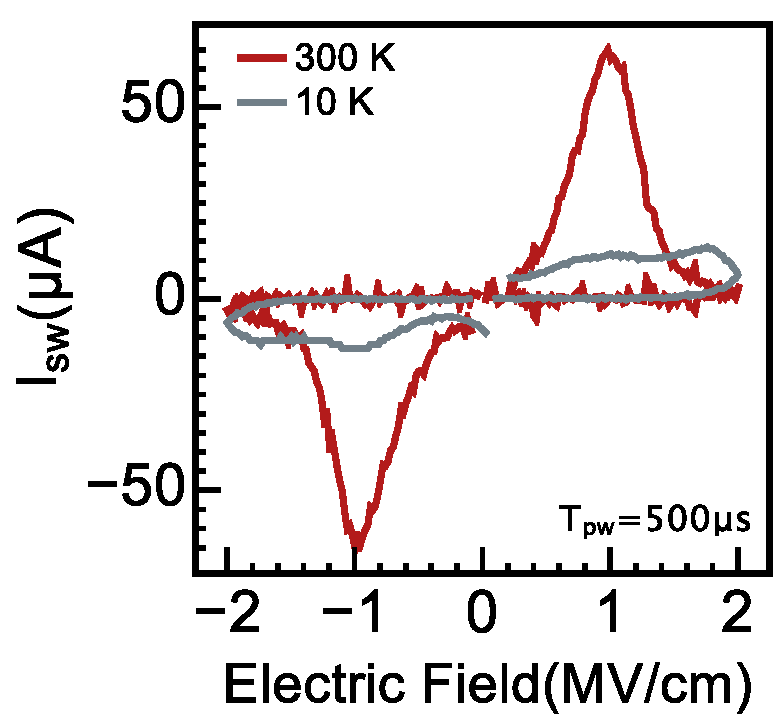
\includegraphics[width=\textwidth]{figures/fig 4a.pdf}
          \caption{}
          \label{fig:fig1a}
     \end{subfigure}
     \hfill
     \begin{subfigure}[b]{0.49\columnwidth}
          \centering
          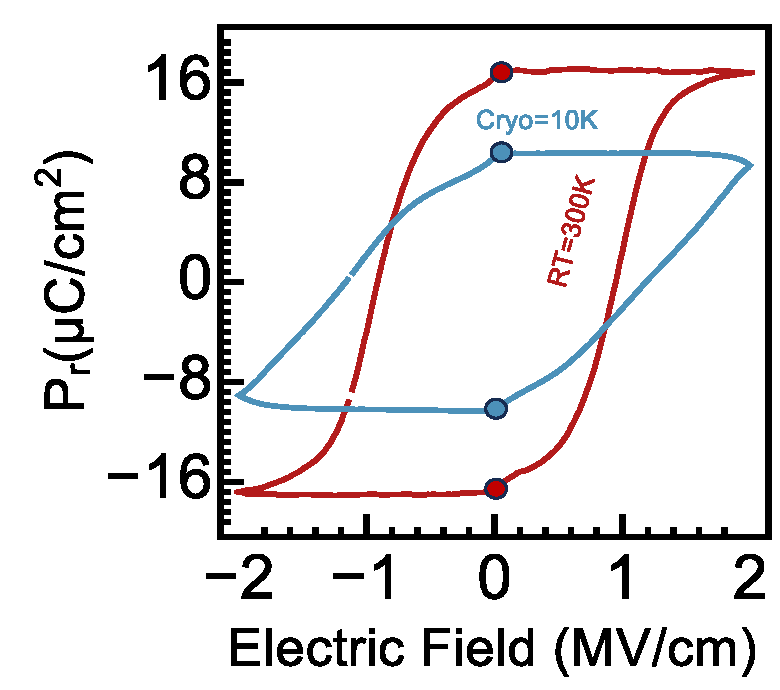
\includegraphics[width=\textwidth]{figures/fig 5b.pdf}
          \caption{}
          \label{fig:fig1b}
     \end{subfigure}
      \hfill
     \begin{subfigure}[b]{0.47\columnwidth}
          \centering
          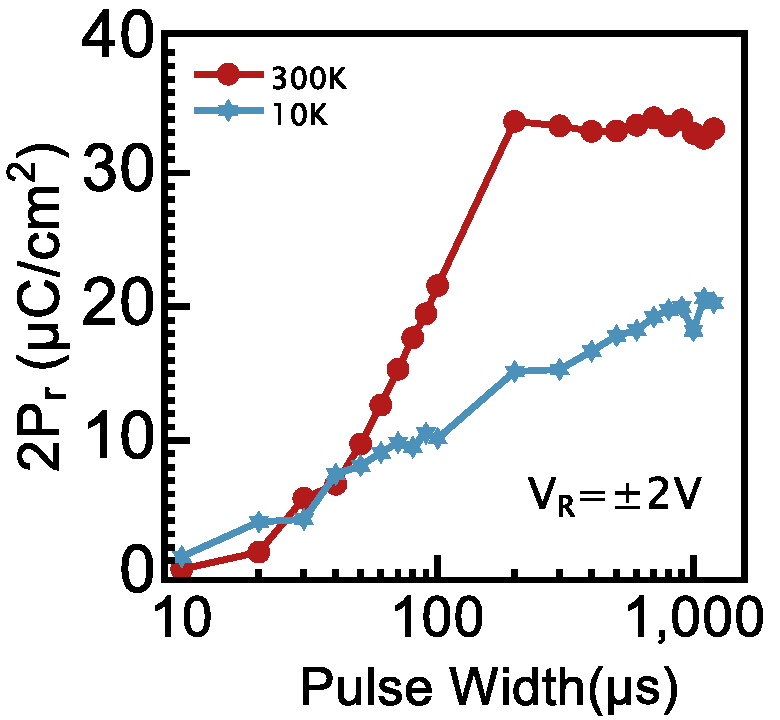
\includegraphics[width=\textwidth]{figures/fig 4c.pdf}
          \caption{}
          \label{fig:fig1c}
     \end{subfigure}
      \hfill
           \begin{subfigure}[b]{0.49\columnwidth}
          \centering
          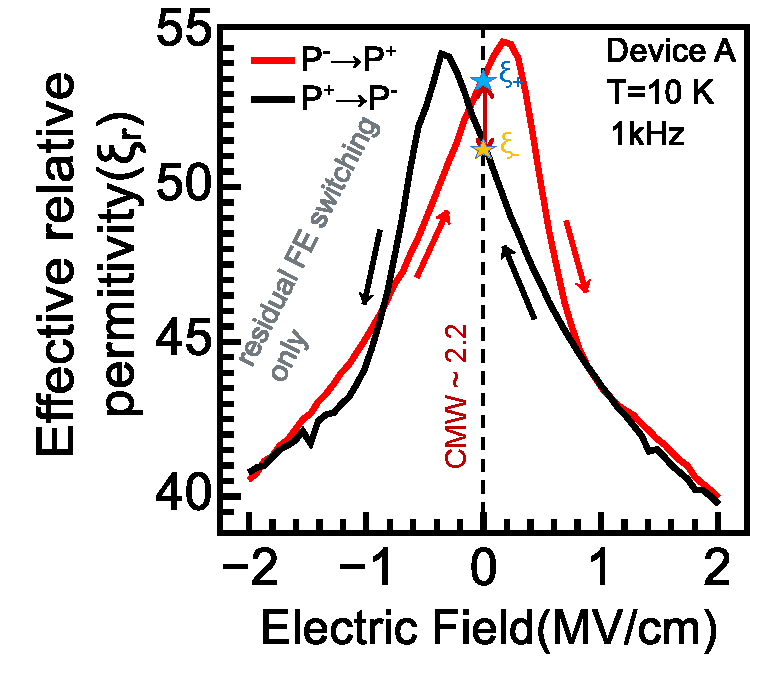
\includegraphics[width=\textwidth]{figures/fig 5d.pdf}
          \caption{}
          \label{fig:fig1c}
     \end{subfigure}
           \hfill
           \begin{subfigure}[b]{0.47\columnwidth}
          \centering
          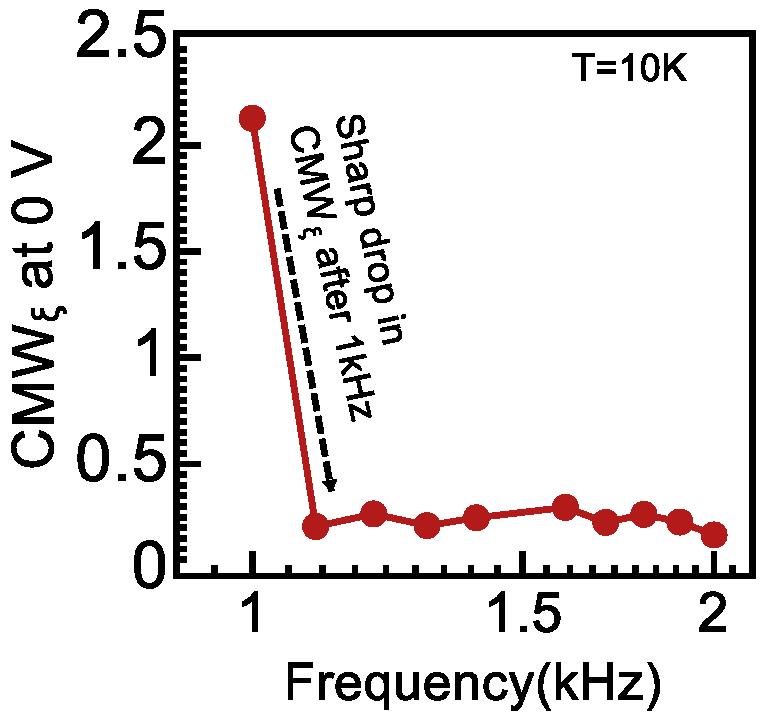
\includegraphics[width=\textwidth]{figures/fig 4d.pdf}
          \caption{}
          \label{fig:fig1c}
     \end{subfigure}
           \hfill
           \begin{subfigure}[b]{0.49\columnwidth}
          \centering
          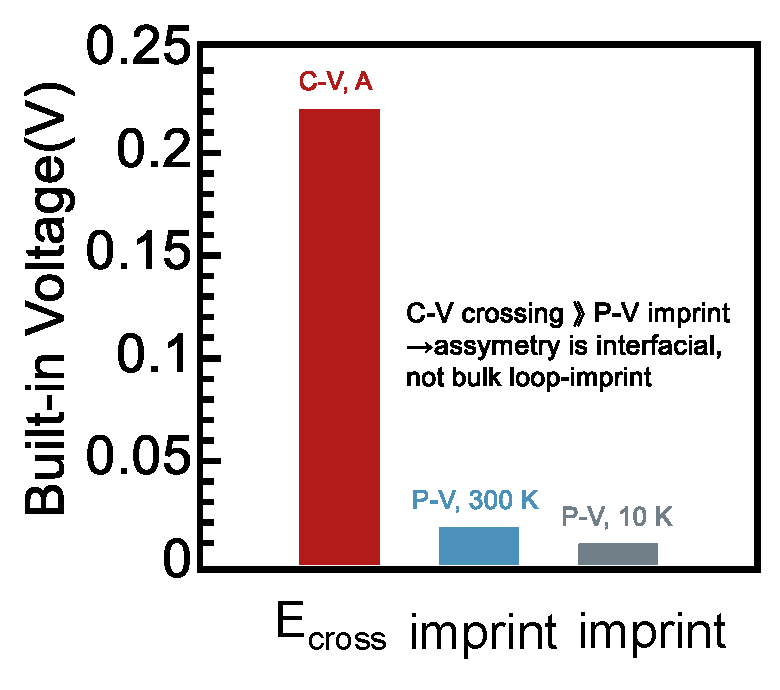
\includegraphics[width=\textwidth]{figures/fig 5e.pdf}
          \caption{}
          \label{fig:fig1c}
     \end{subfigure}
           \hfill
     
     \caption{The window freezes while switching persists (Stack~A). (a) Switching
current at 300~K and 10~K ($T_{pw} = 500\,\mu$s); the peaks fall from
$\pm65\,\mu$A to $\approx13\,\mu$A and shift to higher field, but switching
persists. (b) $P$--$E$ hysteresis; $2P_r$ falls from 33.1 to 20.3\text{ }\mu\text{C/cm}^2$ while
the coercive field $E_c$ rises from 0.93 to 1.17 MV/cm{}. (c) $2P_r$ versus write
pulse width at $V_R = \pm2$~V; at 300~K the polarization saturates at 33\text{ }\mu\text{C/cm}^2$
by 200~$\mu$s, whereas at 10~K it has not saturated even at 1~ms, showing the
reduction in (b) to be kinetically limited rather than a loss of
ferroelectricity. (d) Butterfly $C$--$V$ of Stack~A at 10~K, 1~kHz; the window
is reduced to $\CMW_\xi \approx 2.2$ (from 5.2 at 300~K) but the film still
switches. (e) CMW at 0~V versus frequency at 10~K; the window is resolvable
only at the lowest measured frequency and falls to the noise floor above
1.1~kHz. Since no single relaxation can fall by an order of magnitude across a
10\% frequency interval, this bounds the corner at $f_c \lesssim 1$~kHz---more
than two decades below its 300~K value. (f) Two independent measures of the
internal built-in voltage: the $P$--$E$ loop imprint, $(V_c^+ + V_c^-)/2$, is
only 0.017~V at 300~K and 0.009~V at 10~K, whereas the $C$--$V$ crossing voltage
that closes the window is 0.221~V. Because the built-in field gating the window
is an order of magnitude larger than the one the switching polarization feels,
it cannot reside in the ferroelectric bulk but is localized at the interfacial
layer, which supports a large share of the applied bias while contributing
negligibly to the switched charge.}
     \label{fig:figure1}
\end{figure}



\subsection{Design Rules for Capacitive Readout}
\textit{The usable read band is $f \lesssim \fc(T)$, and it is an interface
property.} Reading above the corner does not merely reduce the margin, it
eliminates it. Since $\fc$ varies from 179~kHz to 1.4~kHz between our two
stacks, a read frequency well inside the plateau for one stack lies two
decades beyond the corner for the other. A CMW quoted at a single frequency
is therefore not portable across stacks, and apparent disagreements between
reports may reflect only where each probe frequency sat relative to that
device's corner. We suggest CMW values be reported together with the measured
$\fc$, or with evidence that the read frequency lies in the plateau.

\textit{A larger zero-bias window trades against stability.} The margin
obtained through interfacial asymmetry is built from the same charge that
relaxes with frequency and freezes on cooling. This gives a physical basis
for the reliability concerns motivating symmetric-stack, finite-read-bias
designs~\cite{lee2025aem,rana2025cp,fehlings2025}: the two philosophies
represent a genuine trade between circuit simplicity and read-margin
stability.

\textit{Capacitive read is a warm-temperature technique.} At 10~K the readout
bandwidth has collapsed below 1~kHz while switching persists, so a
capacitive-read cell that functions at 300~K may fail to resolve its states
at cryogenic temperature. Cryogenic ferroelectric memory should therefore
fall back on the polarization read, which remains available precisely because
the polarization survives---with write pulses lengthened to $\gtrsim$1~ms to
accommodate the slower kinetics of
Fig.~\ref{fig:temperature}(c)~\cite{das2026cryo}.